

\input{../Latex_Templates/Preamble_Report}

%%%%% TITLE PAGE

%\subject{, VT23}
\title{Some relations between equilibria of harmonic vector fields and the domain topology. \\[1ex]
	  \large Master Thesis}
%\subtitle{}
\author{Theo Koppenhöfer}
\date{Lund \\[1ex] \today}

\addbibresource{bibliography.bib}

\usepackage{svg}
\graphicspath{{../Plots/}}
\graphicspath{{../Figures/}}

\usepackage{makecell}
\newcounter{symbolCount}
\newcommand{\nomenclature}[2]{\stepcounter{symbolCount}
\glsxtrnewsymbol[description={#2}]{\arabic{symbolCount}}{#1}}
\usepackage[symbols,
  stylemods={tree},% loads glossaries-extra-stylemods to patch styles
  record, % using 'bib2gls'
  nonumberlist
]{glossaries-extra}

% % assign titles to group labels: 
% \glsxtrsetgrouptitle{latin}{Latin}
% \glsxtrsetgrouptitle{greek}{Greek}

% \GlsXtrLoadResources[
%  src={symbolsList.bib},
%  type=symbols,
% %  group={latin},% assign group label
% %  set-widest,% needed for 'alttree' styles
%  save-locations=false
% ]

% \glsxtrnewsymbol[description={velocity}]{v}{\ensuremath{v}}



% The following displays the labels, uncomment for final version
% \usepackage{showlabels}

\newcommand{\bx}{\bar{x}}
\renewcommand{\chaptername}{Section}

%%%%% The content starts here %%%%%%%%%%%%%


\begin{document}

\maketitle

\tableofcontents

\newpage

\listoftodos

\todoin[]{
  General TODOs
  \begin{itemize}
    \item Check for typos.
    \item Does Girault-Raviart theorem with Helmholtz decomp. help?
    \item bring in results from \cite{Shelton1980} and \cite{Morse1970}
    \item Harmonic vector fields, find up to date reference
    \item Mention Sard's theorem
    \item Does Bocher's theorem help?
    \item Look at application of Sperner's lemma
    \item $C$ is used once for critical points, once for level sets.
    \item Define traversing vector field
    \item Look at regularity requirements. In particular: Riemannian mfs
  \end{itemize}
  Some questions
  \begin{itemize}
    \item Should I state Hopf's Lemma?
    \item Weak formulation - a distraction? \textrightarrow Hartman, Wintner
  \end{itemize}
}

\newpage

\section{Introduction}

\ruggedtodo[inline]{Some amazing introduction}

Unless otherwise stated we denote by $X\subseteq\R^d$ a compact subset of $\R^d$ with boundary $\Sigma=\partial X$ and interior
$\Omega=\interior(X)$.
In the following we will work in dimensions $d\in\brk[c]{2,3}$.
We denote by
\begin{align*}
  f\colon X\to\R
\end{align*}
a scalar function of class $C^2$.
We also denote by
\begin{align*}
  u\colon\overline{\Omega}\to\R^d
\end{align*}
a vector field of class $C^1$.
Often but not always $u$ can be thought of as 
a \emph{harmonic vector field}, that is $u$ is of type $C^1$ and fulfils
\begin{align*}
  \diver u=0 \qquad \text{ and }\qquad \curl u=0\,.
\end{align*}
Also often but not always we assume that globally $u=\nabla f$ is a gradient field, implying that $f$ is harmonic.
One question we seek to answer in this thesis is the following.
\begin{question}[Flowthrough with stagnation point]\label{qu:flowthroughStagnationPoint}
  Does there exist a tube $\Omega\subseteq\R^3$ with flow $u$ through the tube such that
  \begin{enumerate}
    \item $u$ is a harmonic vector field
    \item $u$ has an interior stagnation point
    \item $u$ enters the tube on the one side and exits the tube on the other?
  \end{enumerate}
\end{question}
The answer for this will turn out to be yes for dimensions $d\geq3$ and no for the dimension $d=2$.
In the case of $d=2$ dimensions we will look at what happens if we allow for holes in the domain.
other questions are of the type
\begin{question}[stagnation points of harmonic vector fields without inflow or outflow]
  Let $u$ be a flow in a domain $X$ and such that at every boundary point it is tangential to the boundary.
  What can be said about the relation between the number of critical points and the domain topology?
\end{question}
This question yields a very nice result in the case of $d=2$ dimensions.
To make the formulation of these questions more precise we begin with some general definitions regarding stagnation points and the boundary conditions.

\nomenclature{$d$}{Dimensions $d=2$ or $d=3$}
\nomenclature{$\Omega$}{Domain in $\R^d$, assumed to be $\interior\brk*{X}$}
\nomenclature{$\Sigma$}{Boundary of $\Omega$ or $X$}
\nomenclature{$f\colon X\to\R$}{A $C^2$ mapping, often assumed harmonic}
\nomenclature{$u\colon X\to\R^d\text{ or }T^*\overline{\Omega}$}{A $C^1$ vector field, often assumed harmonic}

\subsection{General definitions}

We start by requiring some regularity for the boundary of $X$.
More precisely we require $X$ to be a compact manifold with corners as in \cite{Handron2002}.
\begin{definition}[Manifolds with corners]
  We introduce the notation
  \begin{align*}
    H_j^d=\R_{\geq0}^j\times\R^{d-j}\subseteq\R^d\,.
  \end{align*}
  A \emph{manifold with (convex) corners} is a topological space $X$ together with an atlas $\cA$ such that for every point
  $x\in X$ there exists an open neighbourhood $U_x$ of $x$, a number $j=j(x)$ and a
  diffeomorphism $\phi\colon U_x\to H_j^d$ in $\cA$ with $\phi(x)=0$.
  We further define sets 
  \begin{align}
    X_k=\brk[c]*{x\in X\colon j(x)=k}\label{eq:def_mfCorners_stratification},
  \end{align}
  which form a stratification of $X$.
\end{definition}
\nomenclature{$X$}{A compact manifold with corners, assumed to be $X=\overline{\Omega}$}
\nomenclature{$Y$}{A manifold}

More generally we give the definition of a stratification as 
\begin{definition}[Stratified space]\label{df:stratified_space}
  A \emph{stratified space} is a collection of a topological space $X$ and a collection of subspaces
  $X_j\subseteq X$, $j\in\cJ$, called \emph{strata},  indexed by a partially ordered set $\cJ$ such that
  \begin{enumerate}
    \item each $X_j$ is a manifold (without boundary) of dimension $n=n(j)$
    \item $X=\bigcup_jX_j$
    \item $X_j\cap \overline{X}_k\neq\emptyset$ iff $X_j\subseteq\overline{X}_k$.
  \end{enumerate}
  In the case that $X_j\subseteq\overline{X}_k$ and additionally $n(j)=0$ or $n(j)=n(k)+1$ we will
  write $X_j\precsim X_k$ or, abusing notation, write $X_k=X_{j-1}$.
\end{definition}
\nomenclature{$X_j$}{A stratification of $X$ as given in definition \ref{df:stratified_space}.
   Often but not always assumed to be given by equation \ref{eq:def_mfCorners_stratification}}

In the case that the stratification arises through relation \eqref{eq:def_mfCorners_stratification}
we have precisely $X_{j}\precsim X_{j-1}$ for $j\in\brk[c]*{1,\dots,d}$ and $X_0\precsim X_0$.

For completeness we also give the definition of the conormal bundle and the contingent cone for a 
stratification $X_j$ of $X$
\begin{definition}[Normal bundle, contingent cone]
  We define the \emph{normal bundle} for a stratification of $X$ to be the quotient space
  \begin{align}
    NX_j=TX_{j-1}/TX_j,
  \end{align}
  where $TX_j$ is the tangent space of $X_j$.
  The \emph{conormal bundle} $N^*X_j$ is defined as its pointwise dual, that is
  \begin{align*}
    N_x^*X_j=\brk*{N_xX_j}'\,.
  \end{align*}
  We define the \emph{contingent cone} (according to Bouligand) for a set $Y\subseteq X$ at $x\in\overline{Y}$ as
  \begin{align}
    C_xY=\brk[c]*{v\in\R^d\colon \text{ there exists }\lambda_n\to0\text{ and }Y\ni x_n\to x\text{ s.t. }
    \lim_n\lambda_n(v-v_n)=0}\,.
  \end{align}
\end{definition}

Given a vector field $u\colon X\to\R^d$ and the above stratification $X_k$ of $X$ we can construct for every
$j\in\cJ$ a vector field
\begin{align*}
  u_j\colon X_j\to T^*X_j\,.
\end{align*}
Here $T^*X_j$ denotes the cotangent space of the manifold $X_j$ as defined for example in \cite[Chapter 6]{Hirsch1994}.
More precisely, for $x\in X_j$ let
\begin{align}
  \pi_j\big\vert_x\colon\R^d\cong T_x^*\R^d\to T_x^*X_{j}\label{eq:def_projectionStratification}
\end{align}
denote the orthogonal projection of a vector at $x$ onto the cotangent space of the stratum $X_j$ at $x$.
Now set
\begin{align}
  u_j=u\big\vert_{T^*X_j}=\pi_j\circ u\big\vert_{X_j}\in C^1\brk*{T^*X_j}\label{eq:def_projectionUStratification}
\end{align}
be the restriction of $u$ onto the cotangent bundle $T^*X_j$.
\nomenclature{$u_j$}{Restriction of $u$ to the cotangent bundle $T^*X_j$, see equation \ref{eq:def_projectionUStratification}}


In the following we define the emergent and the entrant boundary in a way that generalises
\cite[p.282]{Morse1970} for stratified manifolds.
\begin{definition}[Emergent and entrant boundary]\label{df:emergentEntrantBd}
  \td{rewrite the following}
  We call a vector $v\in T_x\R^d$ \emph{entrant} at a boundary point $x\in\Sigma$ iff $v$
  lies in the relative interiour of the polar cone of the contingent cone $C_xX$, that is
  \begin{align*}
    v\in \relint \brk*{C_xX}^o=\brk[c]*{w\in T_xX\colon w\cdot w'<0\text{ for all }w'\in C_xX}
  \end{align*}
  This can be thought of as that $v$ is not tangent to the boundary $\Sigma$ and points into the interiour of $\Omega$.
  Analogously we call $v$ \emph{emergent} iff $v$ belongs to the relative interiour of 
  the dual cone of the contingent cone $C_x\Sigma$, that is
  \begin{align*}
    v\in \relint \brk*{C_xX}^*=\brk[c]*{w\in T_xX\colon w\cdot w'>0\text{ for all }w'\in C_xX}
  \end{align*}
  We define the \emph{entrant boundary} $\Sigma^-$ to be the set of boundary points at which $u$ is entrant.
  Analogously define the \emph{emergent boundary} $\Sigma^+$ to be the set of boundary points at which
  $u$ is emergent.
  Further define the \emph{tangential boundary} $\Sigma^0$ to be
  \begin{align}
    \Sigma^0=\Sigma\setminus\brk*{\Sigma^+\cup\Sigma^-}\cup \partial\Sigma^+\cup\partial\Sigma^-
  \end{align}
  For convenience we also introduce the \emph{non-entrant boundary} $\Sigma^{\geq0}=\Sigma^+\sqcup\Sigma^0$ and the 
  \emph{non-emergent} boundary  $\Sigma^{\leq}=\Sigma^-\sqcup\Sigma^0$.
\end{definition}
\nomenclature{$\Sigma^-$}{entrant boundary, see definition \ref{df:emergentEntrantBd}}
\nomenclature{$\Sigma^+$}{emergent boundary, see definition \ref{df:emergentEntrantBd}}
\nomenclature{$\Sigma^0$}{tangential boundary, see definition \ref{df:emergentEntrantBd}}



\td{illustrate on boundary with corners}
We would now like to illustrate the preceding definitions.
\begin{example}\label{ex:n3_hvf_canonical}
  We now consider our domain to be the ball $B_1\subseteq\R^3$ around the origin in $d=3$ dimensions.
  Now consider the harmonic function
  \begin{equation}
    \begin{aligned}
    f\colon \Omega&\to\R \\
    x&\mapsto x_1^2+x_2^2-2x_3^2\label{eq:n3_hf_canonical}
    \end{aligned}
  \end{equation}
  Which induces the harmonic vector field $u=\nabla f$, or more precisely
  \begin{equation}
    \begin{aligned}
    u\colon \Omega&\to\R \\
    x&\mapsto \vect{2x_1 & 2x_2 & -4x_3}^\top\,.\label{eq:n3_hvf_canonical}
    \end{aligned}
  \end{equation}
  We have that the normal to the boundary $\Sigma=S^2$ is given by
  \begin{align*}
    n\colon S^2&\to S^2 \\
    x&\mapsto x
  \end{align*}
  and thus we have that $x\in\Sigma^-$ iff 
  \begin{align*}
    0>n\cdot u = 2\brk*{x_1^2+x_2^2-2x_3^2}=2f(x)
  \end{align*}
  A plot of the sets can be seen in figure \ref{pl:n3_hvf_canonical_boundary}.
  \begin{figure}
    \centering
    \missingfigure[figwidth=0.7\textwidth]{}
    \caption{Plots of the entrant, emergent and tangential boundary for the
      function $f$ given by equation \eqref{eq:n3_hf_canonical}}
    \label{pl:n3_hvf_canonical_boundary}
  \end{figure}
\end{example}

The following are slight generalisation of definitions given in \cite[p.138f]{Shelton1980}, \cite[§5]{Morse1969} and \cite[p.282f]{Morse1970}
to include harmonic vector fields.\td{Have a closer look at the regularity in the following.}
\begin{definition}[Stagnation points]\label{df:nonDegeneracy}
  Let $u_j\colon X_j\to T^*X_j$ be a $C^1$ vector field on a stratification of $X$.
  We call $x\in X_j$ a \emph{stagnation point} iff $u_{j-1}(x)$ belongs to  the
  polar cone of the contingent
  cone $C_xX_j$ or to the dual cone of the contingent cone $C_xX_j$, that is
  \begin{align*}
    u_{j-1}(x)\in (C_xX_j)^o=\brk[c]*{v\in T_x^*X\colon v\cdot w\leq0 \text{ for all }w\in C_xX_j}
  \end{align*}
  or
  \begin{align*}
    u_{j-1}(x)\in (C_xX_j)^*=\brk[c]*{v\in T_x^*X\colon v\cdot w\geq0 \text{ for all }w\in C_xX_j}\,.
  \end{align*}
  A necessary condition for this is that $x$ is a zero of $u_j$.
  If $X_j$ has dimension $n(j)=d$ then we call $x$ an \emph{interior stagnation point}.
  If $x$ does not lie in the emergent boundary $\Sigma^+$ we call $x$ an \emph{essential stagnation point}.
  The set of all essential stagnation points of $u_j$ is denoted by $\critical_j=\critical_j(u)$.
  A stagnation point $x$ is called
  \emph{non-degenerate} iff 
  \begin{align}
    u_{j-1}(x)\in\relint (C_xX_j)^*\cup \relint (C_xX_j)^o
  \end{align}
  and additionally the derivative
  \begin{align*}
    Du_j(x)=Du_j\big\vert_x\in T_xT^*X\cong \R^{n\times n}
  \end{align*}
  is bijective.
  In addition we say that $x$ has \emph{index} $k$
  if $Du_j(x)$ has exactly $k$ negative eigenvalues.
  $u_j$ is called \emph{(essentially) non-degenerate} if all its stagnation points
  are (essentially) non-degenerate. 
  Assume $u_j$ is non-degenerate then we can define the \emph{$k$-th type number} of the
  stratum $X_j$ to be the number of essential critical points of $u_j$ of index $k$,
  that is
  \begin{align*}
    \ind_{j,k}(u)=\#\brk[c]*{x\in\critical_j(u)\colon x\text{ has index }k}\,.
  \end{align*}
  We define the \emph{interior type numbers} by
  \begin{align*}
    M_k=\sum_{j\colon n(j)=d}\ind_{j,k}(u)\,.
  \end{align*}
  The total number of interior
  stagnation points of $u$ is then given by
  \begin{align*}
    M=\sum_kM_k\,.
  \end{align*}
  \nomenclature{$M_k$}{interior type numbers}
  \nomenclature{$M$}{Total number of stagnation points}
  Analogously we define the \emph{$k$-th boundary type numbers} to be the number of essential boundary 
  stagnation points of $u$ of index $k$, that is
  \begin{align*}
    \mu_k=\sum_{j\colon n(j)<d}\ind_{j,k}(u)
  \end{align*}
  We further write $\nu_k$ for the $k$-th boundary type number of $-u$.
\end{definition}
\nomenclature{$\mu_k$}{boundary type numbers of $f$, see definition \ref{df:bdTypeNbrs}}
\nomenclature{$\nu_k$}{boundary type numbers of $-f$, see definition \ref{df:bdTypeNbrs}}

\begin{definition}[Morse functions]
  We call $u$ \emph{(essentially) Morse} iff for all $j$ we have that $u_j$ is (essentially) non-degenerate.
  For an essentially Morse function $u$ we will denote the number of
  essential stagnation points of $u$ of index $k$ by
  \begin{align*}
    \ind_k(u)=\sum_{j=0}^d\ind_{j,k}(u)=\#\brk[c]*{x\in\bigcup_j\critical_j(u)\colon x\text{ has index }k}\,.
  \end{align*}
\end{definition}

The following definition is inspired by \cite{Katz2014}.
\td{this definition is floating freely, also incorporate strata.}
\begin{definition}[Tangency regular]
  We call a point $x\in\Sigma^0$ a \emph{tangency point}.
  We call a function $u\colon X\to\R^d$ tangency regular iff at every tangency point $x\in\Sigma^0$
  we have that $Du_x(u)\neq0$.
\end{definition}

The previous definitions translate naturally to $f$.
That is we call $f$ Morse, non-degenerate, et cetera iff $u=\nabla f$ is Morse, non-degenerate, et cetera.
Similarly we call $x$ an critical point of $f$ of index $k$ if it is a
stagnation point of $u$ of index $k$.

\tdrewrite{discuss index on manifold with corners.}
To illustrate the preceding definitions we return to our previous example.
\begin{example}
  Let $f$ and $u$ be as in example \ref{ex:n3_hvf_canonical}. One sees from equation \eqref{eq:n3_hvf_canonical}
  that the origin $0$ is the sole interior critical point of $f$. Since we have that
  \begin{align*}
    Du(x) = \begin{bmatrix}
      2 & & \\
       & 2 & \\
      & & -4
    \end{bmatrix}
  \end{align*}
  for all $x\in\Omega$ we see that $Du(0)$ is bijective and thus a non-degenerate critical point. Since $Du(0)$ has
  exactly one negative eigenvalue we see that the origin has index $1$. Since there are no other critical points we have
  $M=1$ and
  \begin{align*}
    M_k=\delta_{k1}\,.
  \end{align*}
  We now calculate for $x\in S^2$
  \begin{align*}
    \tiu(x) = \brk*{u-\brk*{n\cdot u}n}(x)
    = \brk*{u-2f\,n}(x)
    = 2\vect{(1-f(x))x_1 \\(1-f(x))x_2 \\(-2-f(x))x_2}
  \end{align*}
  Hence we see that $x\in\Sigma$ is a critical point iff 
  \begin{align}
    f(x)=1 \text{ and }x_3=0\text{ or } \label{eq:n3_hf_canonical_cps_degenerate} \\
    f(x)=-2 = \text{ and }x_1=0=x_2\,. \label{eq:n3_hf_canonical_cps_nondegenerate}
  \end{align}
  The former equation \eqref{eq:n3_hf_canonical_cps_degenerate} gives that every
  point belonging to $S^1\times\brk[c]{0}\subseteq\R^3$ is in fact a critical point of $f$.
  But since $f=1$ on this set these points are degenerate.
  We will discuss a fix to this issue in the upcoming section.
  We now consider equation \eqref{eq:n3_hf_canonical_cps_nondegenerate} and take 
   $f(x)=-2$ then we must have that $x=\pm e_3$ where $e_k=\delta_{k\cdot}$
  is the $k$-th basis vector in $\R^d$. We now determine their index. For this consider the curves
  \begin{align*}
    \gamma_k\colon\R&\to S^2\\
    t&\mapsto \sin(t)e_k\pm\cos(t)e_3
  \end{align*}
  for $k\in\brk[c]*{1,2}$.
  Note that $\gamma_k'(0)=e_k$ and $\gamma_k(0)=\pm e_3$.
  We see that
  \begin{align*}
    Du(e_1)(\gamma_k'(0))=(u\circ\gamma_k)'(0)
    =\brk*{\sin(t)e_k\mp2\cos(t)e_3}'(0)
    =e_k=\gamma_k'(0)
  \end{align*}
  and thus $e_k\in T_{\pm e_3}S^2$ are eigenvectors of $Du(e_k)$ to eigenvalues $1$.
  Since the $e_k$ span the tangent space $T_{\pm e_3}S^2$ it follows that
  the $\pm e_3$ are non-degenerate critical points of $f$ with index $0$.
\end{example}

\subsection{On assuming non-degeneracy}

\tdrewrite{Use updated notation from previous section. Change for manifolds with corners.}
In the following section we argue that assuming non-degeneracy 
of $u$ and $f$ is not a great restriction.
Given $u$ we define the modification
\begin{align}
  u^\e=u+\e\label{eq:nonDegeneracy:definitionUEps}
\end{align}
\nomenclature{$u_\e$}{modification to $u$ as in equation \eqref{eq:nonDegeneracy:definitionUEps}}
for some $\e\in\R^d$. We would like to show that $u_\e$ is for almost all choices of $\e$ non-degenerate and can 
thus be used to approximate a degenerate $u$.
Our approach is to use Thom's theorem which is inspired by the approach in \cite[Chapter 6]{Hirsch1994}.
In this section we refer to $X$ and $Y$ as generic manifolds without boundary \ruggedtodo{of which class?}.
\begin{definition}[Transversality]
  We call a function $g\colon X\to Y$ transverse to a submanifold $A\subseteq Y$ iff for all points in the 
  preimage $x\in g^{-1}(A)$ we have that
  \begin{align*}
    \Image(Dg_x)+T_{g(x)}A = T_{g(x)}Y\,.
  \end{align*}
\end{definition}
\nomenclature{$A$}{submanifold, can be thought of as the zero section of $T^*X$}
As an application we make the following observation.
\begin{proposition}[Transversal characterisation of non-degeneracy]\label{pr:nonDegeneracy:alternativeCharacterisation}
  Let $u\colon X\to T^*X$ be a differentiable vector field.
  Then $u$ is non-degenerate iff $u$ is transverse to the zero section $A$ of $T^*X$.
\end{proposition}
\begin{proof}
  First note that we have that $x\in u^{-1}(A)$ iff $u(x)=0$ and thus $u^{-1}(A)=C$.
  Unravelling the definition of transversality we get that $u$ is transverse to the zero section iff for all $x\in C=u^{-1}(A)$
  we have that
  \begin{align}
    \Image(Du_x)+T_{u(x)}A = T_{u(x)}TX\,. \label{eq:nonDegeneracy:uTransverse}
  \end{align}
  As $A$ is the zero section we have $T_{u(x)}A=0$ and equation \eqref{eq:nonDegeneracy:uTransverse}
  is equivalent to stating that $Du$ is of full rank. But $Du$ being of full rank at all points
  in $C$ is equivalent to $u$ being non-degenerate.
\end{proof}
A further application is given by the following proposition.
\begin{proposition}[Transversal characterisation of tangency regularity]
  Let $u\colon X\to T^*X$ be a differentiable vector field on a manifold with corners $X$.
  Let $X_j=\partial_jX$ be a stratification of $X$.
  Then $u$ is tangency regular iff $u$ viewed as a section of the normal bundle $N^*X_j$ is transverse to the zero section of $N^*X_j$ for all $j>0$.
  \ruggedtodo{Why do we require $j>0$}
\end{proposition}
\begin{proof}
  \td{Some proof}
\end{proof}
The following version of Thom's transversality theorem is an adaption (i.e.\ weakening) of \cite[Theorem 2.7]{Hirsch1994} to our needs.
\begin{theorem}[Parametric transversality theorem.]
  Let $E,X,Y$ be $C^r$-manifolds (without boundary) and $A\subseteq Y$ a $C^r$ submanifold such that
  \begin{align*}
    r>\dim X-\dim Y+\dim A\,.
  \end{align*}
  Let further $F\colon E\to C^r\brk*{X,Y}$ be such that the evaluation map
  \begin{align*}
    F^\text{ev}\colon E\times X&\to Y \\
    (\e,x)&\mapsto F_\e(x)
  \end{align*}
  is $C^r$ and transverse to $A$.
  Then the set
  \begin{align*}
    \pitchfork(F;A)=\brk[c]*{\e\in E\colon F_\e\text{ is transverse to } A}
  \end{align*}
  is dense.
\end{theorem}
\begin{proof}
  See \cite[Theorem 2.7]{Hirsch1994} for details.
\end{proof}
Using proposition \ref{pr:nonDegeneracy:alternativeCharacterisation} we obtain the corollary
\begin{corollary}
  Let $u\colon X\to T^*X$ be a harmonic vector field on $X$ and let $X_j$ be a stratification of $X$.
   Then for almost every $\e\in\R^d$ we have that
  \begin{enumerate}
    \item $u_j^\e$ given by equations \eqref{} and \eqref{} is non-degenerate\label{co:nonDegeneracy_density_nonDeg}
    \item $u_j^\e$ is tangency regular\label{co:nonDegeneracy_density_tanReg}
  \end{enumerate}
\end{corollary}
\begin{proof}
  Set $r=2$, $E=\R^d$ and $Y=T^*X_j$. We initially set $X=\Omega$.
  We would like to apply the parametric transversality theorem to the function
  \begin{align*}
    F\colon E&\to C^\infty(X,T^*X) \\
    \e&\mapsto u^\e
  \end{align*}
  We note that $F^\text{ev}$ is sufficiently smooth. 
  We need to show that $F^\text{ev}$ is transverse to the
  zero section $A\subseteq T^*X$. Then the parametric transversality theorem 
  yields a dense $E_j\subseteq E$ on which
  $F$ is transverse to $A$.
  For this note that $E\times C = F^{-1}(A)$.
  It then follows for all $(\e,x)\in F^{-1}(A)$ that
  \begin{align}
    \Image\brk*{DF^\text{ev}_{(\e,x)}}=T_xT^*X\label{eq:nonDegeneracy:surjectiveDF}
  \end{align}
  since we have that
  \begin{align*}
    DF^\text{ev}_{(\e,x)}=\begin{bmatrix}
      Du_x\mid \Id_{d\times d}
    \end{bmatrix}
  \end{align*}
  is surjective. 
  Proposition \ref{pr:nonDegeneracy:alternativeCharacterisation}
  now yields that $u^\e$ non-degenerate on $E_j$.
  
  Analogously we set $X=X_j$ in the previous proof and replace
  $u^\e$ with the restriction $u_j^\e$. To show that 
  equation \eqref{eq:nonDegeneracy:surjectiveDF} holds we resort to the fact that
  \begin{align*}
    DF^\text{ev}_{(\e,x)}
    =D\brk*{u_j^\e(x)}_{(\e,x)}
    =D\pi_j\circ \brk*{Du^\e(x)}_{(\e,x)}
  \end{align*}
  is surjective as a concatenation of surjective functions.
  Thus there also exists a dense set $E_\Sigma\subseteq\R$ on which $u^\e_j$ is
  non-degenerate on $X_j$. Now the set
  \begin{align}
    \overline{E}=\cap_j E_j\subseteq\R
  \end{align}
  is dense and
  for every $\e\in\overline{E}$ the function $u^\e$ fulfils condition \ref{co:nonDegeneracy_density_nonDeg}.

  Now to the tangency regularity. 
\end{proof}

As a consequence we get a version of the results in \cite[§2]{Morse1970}.

We call a boundary point $x\in X_j$ on a strata $X_j$ \emph{ordinary} iff $x$ lies
in the interior of $X_j$ and if there exists a stratum $X_{j-1}$ that $x$ is not critical point of $X_{j-1}$.
\begin{proposition}\label{pr:approximationU}
  Assume all stagnation points of $u$ are
  ordinary. Then there exists a positive $\delta>0$ such that
  for (Lebesgue) almost every $\e\in B_\delta$ we have that
  \begin{itemize}
    \item $u^\e$ is non-degenerate
    \item $u^\e$ is tangency regular
    \item there is a one to one relation of the stagnation points in $\Omega$ and $\Sigma$ preserving
      index and the property of being entrant or emergent.
  \end{itemize}
\end{proposition}
\begin{proof}
  We follow \cite[text]{Morse1970}.
  First choose $\delta$ so small that for all stagnation points of $u^\e$ lie in $\Omega$.
  If there did not exist such a $\delta$ we could choose a sequence $\e_n\to0$ in $\R^d$ such 
  that $u^{\e_n}$ had a stagnation point $x_n$ on $\Sigma$. Since $\Sigma$ is compact we can assume that $x_n$ converges
  to a stagnation point $x$. But then $x$ is also a stagnation point of $u$. A contradiction.

  

  We note that since $\overline{\Omega}$ is compact we have that $\nabla u_\e\to \nabla u$ 
  uniformly as $\abs*{\e}\to0$.
  \td{complete proof}
\end{proof}

One of the reasons for introducing boundary tangency is the following proposition 
\begin{proposition}
  Let $u$ be tangency regular.
  \td{Formulate that $\Sigma^0$ is a substratification with desired properties.}
\end{proposition}
\begin{proof}
  Let $u^\e\to u$. Then we have that 
\end{proof}

\section{Some general remarks}

We make the following remarks
\begin{proposition}
  Let $u$ be non-degenerate. Then the number of
  stagnation points is finite.
\end{proposition}
\begin{proof}
  Let $x$ be a non-degenerate stagnation point. Since $Du(x)$ is invertible there exists
  by the inverse function theorem an open neighbourhood $U_x\subseteq\Omega$ of $x$ on which 
  $u$ is bijective. Hence $x$ is the only stagnation point in $U_x$. Let $C$ denote the set of all
  stagnation points of $u$. Then the sets $U_x$ together with
  \begin{align}
    U_C=\R^d\setminus \overline{C}
  \end{align}
  form an open cover of $\overline{\Omega}$. But $\overline{\Omega}$ is compact and thus there exists
  a finite subcover. Since we have for every stagnation point $x\in C$ that
  $x\not\in U_y$ for all other $y\in C\setminus\brk[c]*{x}$ and $x\not\in U_C$ we must have that $U_x$
  is in the finite subcover. Thus it follows that $\#C<\infty$ is finite.
\end{proof}\ruggedtodo[]{This was stated somewhere in Morse1969. Also, what is with the boundary stagnation points}
As a consequence we obtain the following.
\begin{corollary}
  For a non-degenerate $u$ the type numbers $M_0,\dots,M_d$ and the boundary type numbers $\mu_0,\dots,\mu_{d-1}$
  are finite.
\end{corollary}

\td{State the theorem of Sard}

We state Morse's lemma according to \cite[p.145]{Hirsch1994}
\begin{lemma}
  Let $f\colon X\to\R$ be $C^{2+r}$ and $x$ be a non-degenerate
  critical point of index $k$. Then there exists a $C^r$ chart $(\varphi,U)$ at $x$
  such that we have
  \begin{align*}
    f\colon\varphi^{-1}(y)=f(x)-\sum_{j=1}^ky_j^2+\sum_{j=k+1}^dy_j^2\,.
  \end{align*}
\end{lemma}
\td{State proof.}

\td{Bring order into this section.}

\subsection{Betti numbers}

Let $H_k(X;\R)$ denote the $k$-th homology space of $X$.
For an introduction and definition of these we refer the reader to \cite[Chapter 2]{Hatcher2002}.
We define the $k$-th Betti number as the dimension
\begin{align}
  b_k=\dim_\R H_k(X;\R)\,.\label{eq:df_bettiNbrs}
\end{align}
\nomenclature{$b_k$}{Betti number as defined in equation \eqref{eq:df_bettiNbrs}}

We proceed to give examples for Betti numbers of selected connected domains in $\R^d$.
\begin{example}[In flatland]
  In $d=2$ dimensions the $0$-th Betti number counts the number of connected components
  of $\Omega$ and the first Betti number counts the number of holes of this domain.
  All other Betti numbers vanish in $\R^2$.
  More concretely we give the Betti numbers for selected domains in table \ref{tb:n2_domains_bettiNbrs}.
\end{example}

\begin{table}
  \centering
  \renewcommand{\arraystretch}{3}
  \begin{tabular}{c|c|c|c|c}
    Domain & Picture & $b_0$ & $b_1$ & $b_k$, $k\geq2$ \\ \hline
    Disk $D$ & 
    \begin{minipage}{0.1\textwidth}
      \def\svgwidth{\textwidth}
      \input{../Figures/n2_domains_disk.pdf_tex}
    \end{minipage}
    & 1 & 0 & 0 \\
    Annulus $2D\setminus D$ & 
    \begin{minipage}{0.1\textwidth}
      \def\svgwidth{\textwidth}
      \input{../Figures/n2_domains_annulus.pdf_tex}
    \end{minipage}
    & 1 & 1 & 0 \\
    Two holed button & 
    \begin{minipage}{0.1\textwidth}
      \def\svgwidth{\textwidth}
      \input{../Figures/n2_domains_button.pdf_tex}
    \end{minipage}
    & 1 & 2 & 0 \\
  \end{tabular}
  \caption{Betti numbers for selected domains in $\R^2$.}
  \label{tb:n2_domains_bettiNbrs}
\end{table}

\begin{example}[In spaceland]
  In $d=3$ dimensions the $0$-th Betti number counts the number of connected components
  of $\Omega$, the first Betti number counts the number of holes and the second Betti number
  counts the number of bubbles of the domain. All other Betti numbers vanish.
  The Betti numbers for selected domains can be seen in table \ref{tb:n3_domains_bettiNbrs}.
\end{example}

\begin{table}
  \centering
  \renewcommand{\arraystretch}{3}
  \begin{tabular}{c|c|c|c|c|c}
    Domain & Picture & $b_0$ & $b_1$ & $b_2$ & $b_k$, $k\geq3$ \\ \hline
    Ball $B$ & 
    \begin{minipage}{0.1\textwidth}
      \def\svgwidth{\textwidth}
      \input{../Figures/n3_domains_ball.pdf_tex}
    \end{minipage}
    & 1 & 0 & 0 & 0 \\
    Solid torus $S^1\times D$ & 
    \begin{minipage}{0.1\textwidth}
      \def\svgwidth{\textwidth}
      \input{../Figures/n3_domains_torus.pdf_tex}
    \end{minipage}
    & 1 & 1 & 0 & 0 \\
    Ball with bubble $2B\setminus B$ & 
    \begin{minipage}{0.1\textwidth}
      \def\svgwidth{\textwidth}
      \input{../Figures/n3_domains_ballBubble.pdf_tex}
    \end{minipage}
    & 1 & 0 & 1 & 0 \\
    \makecell{Ball with bubble \\in shape of torus} & 
    \begin{minipage}{0.1\textwidth}
      \def\svgwidth{\textwidth}
      \input{../Figures/n3_domains_ballTorusHole.pdf_tex}
    \end{minipage}
    & 1 & 1 & 1 & 0 \\
  \end{tabular}
  \caption{Betti numbers for selected domains in $\R^3$.}
  \label{tb:n3_domains_bettiNbrs}
\end{table}

\td{Comment on the finiteness of Betti numbers. Check numbers for ball with torus bubble.}

\subsection{The Morse inequalities}

We state the Morse inequalities.\ruggedtodo[]{More citations.}
\begin{theorem}[Strong Morse inequalities]
Let $X$ be a manifold with corners and $f\colon X\to\R$ be essentially Morse.
Then we have for $k\in\brk[c]*{0,\dots,d}$ the inequalities
\begin{align*}
  \sum_{j=0}^k \brk*{-1}^{j+k}\essind_j(f)\geq \sum_{j=0}^k\brk*{-1}^{k+j}b_j(X)\,.
\end{align*}
For $k=d$ we in fact have equality
\begin{align*}
  \sum_{j=0}^d \brk*{-1}^{j}\essind_j(f)= \chi(X)
\end{align*}
where the Euler characteristic
\begin{align*}
  \chi(X)=\sum_{j=0}^d\brk*{-1}^{j}b_j(X)
\end{align*}
is the alternating sum of the Betti numbers.
\end{theorem}
\begin{proof}
  See \cite[Theorem 10.2']{Morse1969}.\ruggedtodo[]{Give outline of proof idea. The citation for this version is no longer up to date.}
\end{proof}

\begin{corollary}[Weak Morse inequalities]
  Let $X$ be a manifold with corners and $f\colon X\to\R$ essentially Morse. Then we have for $k\in\brk[c]*{0,\dots,d}$
  the inequalities
  \begin{align*}
    \essind_k(f)\geq b_k(X)\,.
  \end{align*}
\end{corollary}
\begin{proof}
  \td{Write some proof.}
\end{proof}
If we now assume that $f$ is harmonic then the maximum principle implies that
$M_0=0=M_d$.
If we additionally assume that we have dimensions $d=2$ we obtain \cite[Corollary 10.1]{Morse1969}.
\begin{corollary}[Morse inequalities for $f$ harmonic, $d=2$]
  Let $d=2$, $\Omega$ and $f$ be regular and assume that $f$ is harmonic. Then we have
  \begin{align*}
    \mu_0&\geq b_0 \\
    M+\mu_1-\mu_0&=b_1-b_0\,.
  \end{align*}
\end{corollary}
In dimensions $d=3$ we obtain \cite[Corollary 10.2]{Morse1969}
\begin{corollary}[Morse inequalities for $f$ harmonic, $d=3$]
  Let $d=3$, $\Omega$ and $f$ be regular and assume that $f$ is harmonic. Then we have
  \begin{align*}
    \mu_0&\geq b_0 \\
    M_1+\mu_1-\mu_0&\geq b_1-b_0 \\
    M_2+\mu_2-M_1-\mu_1+\mu_0&= b_2-b_1+b_0\,.
  \end{align*}
\end{corollary}
\ruggedtodo[inline]{Give a classical example of a Morse function to determine the Betti numbers.}
\td{Give an outline of the proof.}

\subsection{On harmonic vector fields}

In the following we deduce some basic relations for harmonic vector fields in dimensions $d\in\brk[c]{2,3}$.
\begin{proposition}[Harmonic vector fields on simply connected domains]\label{pr:n2:hvf:simplyConnected}
  Let $\Omega\subseteq\R^d$ be open and simply connected and $u$ be a harmonic vector field. Then
  \begin{enumerate}
    \item 
    $u=\nabla f$ is the gradient field of some
    function $f\colon\Omega\to\R$.
    \item  $f$ is harmonic.
    \item $u$ is in fact $C^\infty$.
    \item The components $u_i=\partial_if$ are harmonic.
  \end{enumerate}
\end{proposition}
\begin{proof}
  \begin{enumerate}
    \item 
    Since $\curl u =0$ this is a direct consequence of Stokes theorem.
    \item This follows from $\Delta f = \diver u=0$.
    \item This follows from the fact that $f$ is harmonic
    \item This follows from $u_i=\partial_if$.
  \end{enumerate}
\end{proof}

If one considers not necessarily simply connected domains $\Omega$ then we obtain the previous
properties at least locally.

\newpage

\section{Harmonic functions, $d=2$}

The following result is essentially a negative to question \ref{qu:flowthroughStagnationPoint} in $d=2$ dimensions.
\begin{proposition}\label{pr:n2:hf:nonExistence}
  Let $\Omega$ be homeomorphic to $B_1\subseteq\R^2$. Let further $f\colon\overline{\Omega}\to\R$ be regular harmonic  
  with critical point $x_1\in\Omega$. Then $\Sigma^-\subseteq\Sigma$ is not connected.
\end{proposition}
We shall give two different proofs of this result. One involving level-sets and the other involving invariant manifolds

\subsection{A proof involving level-sets}

\ruggedtodo[]{write omega-limit.}
\begin{proof}[Sketch of Proof.]
  Let $y_c=f(x_1)$ and $x_1,\dots,x_M$ be all the critical points such that $f(x_\cdot)=y_c$.
  We claim that the level set
  \begin{align*}
    C=\brk[c]*{f=y_c}\subseteq\overline{\Omega}
  \end{align*}
  can be represented by a multigraph $G$
  which divides the boundary $\Sigma$ into 4 components. To show this let $\gamma_i\colon \brk*{a_i,b_i}\to C$ for $i\in\brk[c]{1,\dots,4}$ parametrise the curves in
  $C$ intersecting at $x_1$. These can be constructed with the initial value problem
  \begin{align*} 
    \gamma'&=\brk*{\nabla f}^\perp\big\vert_\gamma \\
    \gamma(0) &= \gamma_0
  \end{align*}
  where $\gamma_0\in C$ is chosen sufficiently near $x_1$. We assume that the intervals on which the $\gamma_i$ are
  defined are maximal. We thus have for
  \begin{align*}
    \gamma_i^-=\lim_{t\to a_i}\gamma(t) \\
    \gamma_i^+=\lim_{t\to b_i}\gamma(t)
  \end{align*}
  that $\gamma_i^\pm\in\brk[c]*{x_1,\dots,x_M,\Sigma}$ since the $x_j$ are the sole points on $\Omega\cap\overline{C}$
  at which $\nabla f^\perp=0$. This argument can be applied to all of the 
  $x_1,\dots,x_M$. We therefore have a situation similar to the one depicted in figure \ref{fi:n2:levelSets:overview}.
  
  \begin{figure}
    \centering
    \def\svgwidth{0.8\textwidth}
    \input{../Figures/n2_levelSets_overview.pdf_tex}
    \caption{The situation at hand: The edges represent level curves and the interior vertices critical points.}
    \label{fi:n2:levelSets:overview}
  \end{figure}

  Thus $C$ can be represented by a multigraph $G$ with vertices $v_1,\dots,v_K$ and edges $e_1,\dots,e_L\subseteq C$.
  In the following we identify the graph $G$ with its planar embedding in $\overline{\Omega}$.
  Assume $G$ contains a cycle with vertex sequence $v_{i_1},\dots,v_{i_J}$ and edges $e_{i_1},\dots,e_{i_J}$. Then
  \begin{align*}
    \partial E = \bigcup_j e_{i_j}\subseteq C
  \end{align*}
  is the boundary of a domain $E$ for which $f=y_c$ on $\partial E$. By the maximum principle $f=y_c$ on $E$ and thus
  $f=y_c$ on $\overline{\Omega}$, a contradiction to the non-degeneracy. Hence $G$ is acyclic and the number of 
  intersections of $C$ with the boundary $\Sigma$ is at least four and thus the boundary $\Sigma$ is divided into at least four components.
  
  Now choose four neighbouring components $\omega_1,\dots,\omega_4$ as depicted in figure \ref{fi:n2:levelSets:neighbouringComponents}
  \begin{figure}
    \centering
    \input{../figures/n2_levelSets_selectionOmega.pdf_tex}
    \caption{The choice of $\omega_1,\dots,\omega_4$.}
    \label{fi:n2:levelSets:neighbouringComponents}
  \end{figure}
  Let $A\subseteq\Omega$ be the domain bounded
  by $\omega_1$ and $C$ as in the figure. The maximum principle yields that $\omega_1$ contains a local maximum or minimum of $f$ since
  $f=y_c$ is constant on the other boundaries $\partial A\setminus\omega_1$.
  By the same argument $\omega_2,\dots,\omega_4$ also contain local extrema. 
  \ruggedtodo[]{use argument with $\nabla f$ here to show that extrema can be assumed to be alternating.}
  Since the $\partial\omega_i$ cannot be extremal points on $\Sigma$
  we can assume without loss of generality (by switching $f$ for $-f$) that $\omega_1$ and $\omega_3$ contain local maxima and $\omega_2 $ and $\omega_4$ local
  minima. By Hopf's lemma we thus have
  \begin{align*}
    \Sigma^-\cap\omega_2\neq\emptyset\neq\Sigma^-\cap\omega_4
  \end{align*}
  and 
  \begin{align*}
    \Sigma^+\cap\omega_1\neq\emptyset\neq\Sigma^+\cap\omega_3
  \end{align*}
  From this the claim follows.
\end{proof}

\subsection{A proof involving invariant manifolds}

Using invariant manifolds we obtain the following proof.

\begin{proof}[Sketch of Proof.]
  Let $x_1,\dots,x_M$ denote the critical points of $f$. Let $\lambda_i\colon\brk*{a_i,b_i}\to\overline{\Omega}$ for $i\in\brk[c]{1,2}$ parametrise the unstable manifolds of the
  critical point $x_1$ and
  $\lambda_i\colon\brk*{a_i,b_i}\to\overline{\Omega}$ for $i\in\brk[c]{3,4}$ be chosen to parametrise the stable manifolds of $x_1$.
  As in the previous proof we can assume the interval on which the $\lambda_i$ are defined to be maximal. We thus have for
  \begin{align*}
    \lambda_i^-=\lim_{t\to a_i}\lambda(t) \\
    \lambda_i^+=\lim_{t\to b_i}\lambda(t)
  \end{align*}
  that $\lambda_i^\pm\in\brk[c]*{x_1,\dots,x_M,\Sigma}$ since the $x_j$ are the sole points on $\overline{\Omega}$
  at which $Df=0$. Thus all invariant manifolds of all critical points form a directed multigraph $G$ with vertices $v_1,\dots,v_K$ and 
  edges $e_1,\dots,e_L\subseteq\overline{\Omega}$. Here the direction of the edge is determined by whether $f$ increases or decreases
  along the edge.
  Once again we identify the graph with its planar embedding.
  By construction graph is acyclic directed. We claim that the underlying undirected graph is in fact a forest. Thus it remains to
  be shown that the underlying undirected graph is acyclic.
  Assume not, i.e.\ we have a undirected cycle A with vertices $x_{i_1},\dots,x_{i_J}$ and edges $e_{i_1},\dots,e_{i_J}$.
  The set of cycles forms a partial ordering with respect to the property `contains another cycle'.
  \ruggedtodo[]{More precise.}
  We can assume that our chosen cycle A
  contains no other distinct cycles, i.e.\ it is a minimal cycle.
  We note that each vertex has 2 incoming and 2 outgoing arcs which lie opposite to one another.
  We also note that the edges cannot cross. 
  We can thus describe the trail $x_{i_1},\dots,x_{i_J}$ by a set of directives of the type
  \begin{align*}
    (d_1,\dots,d_K) \in \brk[c]*{\text{l},\text{r},\text{s}}^J\,.
  \end{align*}
  Here l, r and s stand for `left', `right' and `straight' respectively.
  The underlying idea is that we follow a particular trail and orient all vertices as in figure \ref{fi:n2:invariantMF:directivesDefinition}.
  
  \begin{figure}
    \centering
    \begin{minipage}{0.4\textwidth}
      \def\svgwidth{0.7\textwidth}
      \input{../Figures/n2_invariantMF_directivesDefinition.pdf_tex}
      \caption{Explanation of the directives `l',`r' and `r'.}
      \label{fi:n2:invariantMF:directivesDefinition}
    \end{minipage}
    \hfill
    \begin{minipage}{0.4\textwidth}
      \def\svgwidth{1\textwidth}
      \input{../Figures/n2_invariantMF_directivesExample.pdf_tex}
      \caption{An example for a cycle.}
      \label{fi:n2:invariantMF:directivesExample}
    \end{minipage}
  \end{figure}

  An example of the trail `srsr' is given in figure \ref{fi:n2:invariantMF:directivesExample}.
  We now note that cycles of the type r,\dots,r or l,\dots,l
  cannot occur as we otherwise would have a directed cycle. Thus there exists a vertex where the chosen direction is s. 
  Without loss of generality this vertex is $x_{i_1}$.
  Since we can swap $f$ with $-f$ we can assume without loss of generality that the cycle lies to right of $x_{i_1}$.
  Now consider new cycle B starting at $x_{i_1}$ with directives r,\dots,r.
  Since all vertices of B lie within the cycle A we must at some step reach a vertex on the cycle A. But then cycle B is a new distinct cycle
  contained in cycle A, a contradiction to the minimality of A.
  Hence every case considered leads to a contradiction and it follows that the underlying undirected multigraph of $G$
  is acyclic.
  
  Now call a leaf positive if it lies on the emergent boundary and
  negative if it lies on the entrant boundary. The case that a leaf is neither positive or negative cannot occur.\ruggedtodo[]{elaborate}
  We now pick a tree $\widetilde{G}$ out of $G$ and note that
  there are at least 4 boundary vertices to this tree.
  By construction we see that each `neighbouring'\ruggedtodo[]{elaborate} leaf of this tree
  has opposite signage and the claim follows.
\end{proof}

\subsection{A proof involving Morse theory}

\td{fix the following proof}

% We start with a technical lemma
% \begin{lemma}
%   Let $u\colon\R^{d}\supset (-\eta,\eta)\times U_0\to\R^d$ be a vector field on an open set $U_0\subset\R^{d-1}$. Assume that on $U$ we
%   have that $u\colon e_1>\delta$ on $\brk[c]{0}\times U_0$ for some $\delta>0$. Then we have for almost every $\e>0$ that $u$ restricted to the cotangent space
%   $T^*U_\e$ is Morse. Here the submanifold $U_\e$ is given as 
%   \begin{align}
%     U_\e=\e\graph(\phi)
%   \end{align}
%   for some suitable function $\phi\in C_c^\infty(U_0;[0,1])$.
% \end{lemma}
% \begin{proof}
%   Let $x_0\in U_0$ be degenerate.
% \end{proof}
% For the following proof we require the following technical lemma
% \begin{lemma}
%   Let $X$ be a $d$ dimensional manifold with boundary and $u\colon X\to\R^d$ a smooth Morse vector field. Assume that $\Gamma\subset X$ is
%   $d-1$ dimensional manifold with boundary not containing any interior critical points of $u$ on $X$ and let $\e>0$. Then there exists a manifold $\Gamma_\e\subseteq U_\e\brk*{\Gamma}$ contained
%   in an $\e$ neighbourhood of $\Gamma$ such that $\partial\Gamma=\partial\Gamma_\e$ and such that $f$ is morse on
%   $\interior(\Gamma_\e)$.
% \end{lemma}
% \begin{proof}
  % Let $x$ be a critical point of $u$ on $\Gamma$. Since $x$ is not an interior critical point there exists a neighbourhood $U\subseteq\Gamma$ of 
  % $x$ such that the normal $n\colon U\to \R^d$ is defined, $\abs*{u\cdot n}>\delta$ for some $\delta>0$ and $\abs{n-n(x)}\leq\delta$.
  % Let $r>0$ such that $B_r(x)\cap\Gamma\subseteq U$. We choose a function $\phi\in C_c^\infty(B_r(x);[0,1])$ such that $\phi(x)\neq0$.
  % Define for $\eta>0$
  % the manifold $\Gamma_\eta=\Gamma+\eta\phi n(x)$. We now claim that for almost all $\eta\leq\e$ the function 
  % \begin{align}
  %   \phi\in C_c^\infty(U;\R)
  % \end{align}
  % and require $\phi(x)\neq0$. Now consider the function given by
  % \begin{align}
  %   G(x,t)=\Phi(x,\eta\phi(x)t)
  % \end{align}
  % where $\eta>0$ and $\Phi$ is the flow induced by the vector field $u$. We note that by construction for every $t$ the set
  % \begin{align}
  %   \Gamma\setminus U\cup \image(G(\cdot,t))
  % \end{align}
  % is a smooth manifold.
%   Our aim is to apply the parametric transversality theorem. 
%   Let $x_0$ be a critical point on $\Gamma$. Let $U_0\subseteq\Gamma$ be an open neighbourhood of $x_0$ and
%   let $\phi_0\colon U_0\to U\subseteq\R^{d-1}$ be a chart. Define further the map
%   \begin{align}
%     \Phi_\e(x)=\Phi(x,f(\e,x))\,.
%   \end{align}
%   Here $\Phi$ denotes the flow induced by $u$ and $f\colon E\times U_0\to\R$ is a suitable function (think bump function).
%   Set $\Psi_\e=\Phi_\e^{-1}$, $x_\e=\Phi_\e(x_0)$ and $U_\e=\Phi_\e(U_0)$.
%   Set $\phi_\e=\phi_0\circ\Psi_\e$ and
%   \begin{align}
%     u_\e = D_x\phi_\e\circ\pi_\e\circ u\circ\phi_\e^{-1}
%   \end{align}
%   where $\pi_\e$ is the restriction onto $T^*U_\e$. We now calculate
%   \begin{align}
%     D_\e u_\e=D_\e D_x\phi_\e+D_x\phi_\e D_e\pi_\e+D_x\phi_\e \pi_\e Du D_\e\phi_\e^{-1}
%   \end{align}
%   where we used the linearity of $D_x\phi_\e$ and $\pi_\e$.
%   We now calculate
%   \begin{align}
%     \Id_{E\times T^*U_\e} &=D_{(\e,x)}\vect{\cdot_1&\Phi_{\cdot_1}(\cdot_2)}\circ\vect{\e&\Psi_\e(x)} \\
%     &=\begin{bmatrix}
%       \Id_E&0\\
%       D_\e\Phi_\e(x) & D_x\Phi_\e(x)
%     \end{bmatrix}
%     \begin{bmatrix}
%       \Id_E &0 \\
%       D_\e\Psi_\e(x) & D_x\Psi_\e(x)
%     \end{bmatrix} \\
%     &= 
%     \begin{bmatrix}
%       \Id_E &0 \\
%       D_\e\Phi_\e(x)+D_x\Phi_\e(x)D_\e\Psi_\e(x) & D_x\Phi_\e(x)D_x\Psi_\e(x)
%     \end{bmatrix}
%   \end{align}
%   Thus in particular
%   \begin{align}
%     D_x\Psi_\e=\brk*{D_x\Phi_\e}^{-1}
%   \end{align}
%   Now notice that
%   \begin{align}
%     D_\e\Phi_\e(x)
%     =D_t\Phi D_\e f(\e,x)=u D_\e f 
%   \end{align}
%   and
%   \begin{align}
%     D_x\Phi_\e
%     =D_x\Phi + D_t\Phi D_x f=D_x\Phi + u \otimes D_x f
%   \end{align}
%   by the property of the flow.
  
%   Hence
%   \begin{align}
%     D_x\phi_\e=D\phi_0 D_x\Psi_\e
%   \end{align}
%   which implies
%   \begin{align}
%     D_\e D_x\phi_\e=D^2\phi_0\brk*{D_x\Psi_\e,D_x\Psi_\e}+D\phi_0 D_\e D_x\Psi_\e
%   \end{align}
%   We also see
%   \begin{align}
%     D_\e\phi_\e^{-1}=D_\e\brk*{\Phi_\e\circ\phi_0^{-1}}
%     =D_\e\Phi_\e D\phi_0^{-1}
%   \end{align}

%   Now we look at $\pi_\e$. This is given as 
%   \begin{align}
%     \pi_\e(u)=\sum_i\partial^\e_i(e_i)\cdot u\partial^\e_i
%   \end{align}
% \end{proof}

\begin{proof}
  Assume that $\Sigma^-$ is connected. Then we can cut the domain along $\Gamma$ such that the endpoints
  of the cut coincide with the endpoints of $\Sigma^-$, that is $\partial\Gamma=\partial\Sigma^-$.
  Now we obtain two new domains $X^+$ and $X^-$ such that $\partial X^+ =\Sigma^+\cup\Sigma^0\cup\overline{\Gamma}$ and
  $\partial X^-=\Sigma^-\cup\overline{\Gamma}$. We can assume that $\Gamma$ is a smooth manifold and corresponds to the stratum 
  $X_\Gamma$ for $X^+$ and $X^-$. We also assume that the corner points $x_1,x_2\in\partial\Gamma$ correspond to the strata $X_{1}$ and $X_{2}$.
  For the following argumentation we require that $u$ is Morse on both $X^+$ and $X^-$ so assume this is the case.
  Locally around the corner point $x_1$ we have a situation depicted as in figure \ref{}
  \begin{figure}
    \centering
    \input{../Figures/n2_cutOmega_flowthrough.pdf_tex}
    \caption{The situation at hand.}
    \label{}
  \end{figure}
  That is $u=\nabla f$ is essentially parallel to the boundary $\Sigma$.
  We assume that we chose $\Gamma$ such that the acute angle is on the side where $u$ flows into the new domain.
  Thus we have that $x_1$ is not a critical point of either $f$ nor $-f$.
  Analogously we can choose $\Gamma$ in such a way around $x_2$.
  We now focus our attention on $X^+$. Since no essential critical points lie on $\Sigma^+$ or
  $\partial\Gamma$ it follows for the boundary type numbers that
  \begin{align}
    \mu^+_j=\ind_{\Gamma,j}(f)\,.\label{eq:n2_disproof_morse_muplus}
  \end{align}
  Analogously we have on $X^-$ that
  \begin{align}
    \nu^-_j=\ind_{\Gamma,j}(-f)\,.\label{eq:n2_disproof_morse_numinus}
  \end{align}
  In addition we have that the emergent critical points of $f$ on $X^+$ are the
  entrant critical points of $-f$ on $X^-$, that is
  \begin{align}
    \ind_{\Gamma,0}(f)=\ind_{\Gamma,1}(-f)\qquad\text{ and }\qquad 
    \ind_{\Gamma,1}(f)=\ind_{\Gamma,0}(-f)\label{eq:n2_disproof_morse_relationIndex} 
  \end{align}
  Using equations \eqref{eq:n2_disproof_morse_muplus}, \eqref{eq:n2_disproof_morse_numinus} and \eqref{eq:n2_disproof_morse_relationIndex}
  we obtain
  \begin{align}
    \mu^+_0=\nu^-_1 \qquad\text{ and }\qquad \mu^+_1=\nu^-_0\,.\label{eq:n2_disproof_morse_relationMuNu}
  \end{align}
  Consider the Morse inequality for $f$
  \begin{align}
    M^++\mu^+_1-\mu^+_0=-\chi(X^+)=-\chi(X)\,.\label{eq:n2_disproof_morse_morseineqplus}
  \end{align}
  and the Morse inequality for $-f$
  \begin{align}
    M^-+\nu^-_1-\nu^-_0=-\chi(X^-)=-\chi(X)\,.\label{eq:n2_disproof_morse_morseineqminus}
  \end{align}
  We now add equations \eqref{eq:n2_disproof_morse_morseineqplus} and \eqref{eq:n2_disproof_morse_morseineqminus}
  and insert relations \eqref{eq:n2_disproof_morse_relationMuNu} to obtain
  \begin{align*}
    M^-+M^+=-2\chi(X)<0
  \end{align*}
  in contradiction to $M^\pm\geq0$.

  % The statement now remains to be shown for $u$ which are not Morse on $\Gamma$.
  % By proposition \ref{} we can approximate such $u$ by a sequence $u^\e$ which are
  % Morse on the stratification
  % $$\brk[c]*{X_j}_{j\in\cJ}\cup\brk[c]*{X_\Gamma}\cup\brk[c]*{X_j}_{j\in\brk[c]*{1,2}}$$
  % of $X$. Again by proposition \ref{} we have that $\Sigma^0(u^\e)\to\Sigma^0(u)$ for $\e\to0$.
  % This implies that if we choose the cut $\Gamma^\e$ for $u^\e$ as in figure \ref{}
  % we obtain that for all $u^\e$ all 
\end{proof}
% \begin{proposition}
%   Let $X$ be a simply connected manifold with corners and $f\colon X\to\R$ harmonic and Morse. 
%   Assume further that $\Sigma^-$ is connected. Then $f$ cannot have an interior critical point.
% \end{proposition}
% \begin{proof}
%   Since $\Sigma^-$ is connected we can cut the domain along a cut $\Gamma$ such that the endpoints $\partial\Gamma$ of
%   $\Gamma$ coincide with the endpoints of $\Sigma^-$. Thus we obtain two domains $X^+$ and $X^-$ with boundaries
%   $\partial X^+=\Gamma\cup\Sigma^{\geq0}$ and $\partial X^-=\Gamma\cup\Sigma^-$.
%   On $X^+$ we obtain the Morse inequalities 
% \end{proof}
% \subsubsection*{A proof involving the argument principle}

% \begin{proposition}
%   Let $X$ be a simply connected manifold with corners and $f\colon X\to\R$ harmonic with an
%   interior critical point.
%   Then $\Sigma^-$ is not connected.
% \end{proposition}
% \begin{proof}
%   Assume not.
%   Let $h\in\Hol(X)$ be the holomorphic function given by $h=\nabla f$.
%   Let $\gamma\colon \R\supseteq (t_0,t_2) \to\Sigma$ traverse the boundary of $X$ such that
%   the interior of $X$ lies to the left of $\gamma$.
%   Without loss of generality $\gamma(t_0)$ is the point where $\gamma$ enters the entrant boundary $\Sigma^-$.
%   Let $\gamma(t_1)$ denote the point at which $\gamma$ leaves the entrant boundary $\Sigma^-$.
%   As $\gamma$ traverses $\Sigma^-$ we have that $h$ points into $\Omega$ and thus lies to the left of
%   the tangent $T_\gamma X$. Thus we obtain for the change in argument of $\arg h$ that
%   \begin{align*}
%     \arg h(\gamma(t_1))-\arg h(\gamma(t_0))=\gamma'(t_0)-\gamma'(t_1)+\pi k
%   \end{align*}
%   where $k\in\brk[c]{-1,0,1}$. Similarly we obtain for the change in argument of $\arg h$ as $\gamma$ traverses
%   $\Sigma^+\cup\Sigma^0$ that
%   \begin{align*}
%     \arg h(\gamma(t_2))-\arg h(\gamma(t_1))=\gamma'(t_2)-\gamma'(t_1)+\pi k
%   \end{align*}
%   We then obtain with the argument principle
%   \begin{align*}
%     2\pi M=\int_{\partial X}\dif{\arg(h(z))}
%   \end{align*}
% \end{proof}

\subsection{Allowing for Inflow and outflow}

The strategy in the above proofs can be generalised to show the following
\begin{conjecture}
  Let $X\subseteq\R^2$ be a manifold with corners with Betti numbers $b_0=1$ and $b_1$.
  Let further $f\colon X\to\R$ be Morse harmonic with $M$ critical points.
  Assume that 
  $\overline{\Sigma^-}\subseteq\Sigma$ on a given connected component 
  of the boundary $\Sigma$
  consists of at most one connected component. Then we have
  \begin{align*}
    \frac{4}{3}M\leq b_1+1\,.
  \end{align*}
\end{conjecture}
This inequality can probably be improved considerably.

Let $J^\pm$ denote the number of connected components of $\Sigma^\pm$.
Consider a disjoint decomposition of the boundary $\Sigma=\Sigma_{\geq0}\sqcup\Sigma_{\leq0}$ such
that $\Sigma_{\geq0}\subseteq\Sigma^{\geq0}$ and $\Sigma_{\leq0}\subseteq\Sigma^{\leq0}$.
Let now $J^{\geq0}$ denote the minimal number of connected components of $\Sigma^{\geq0}$ of all such
decompositions.
We state a consequence of a result from \cite[Theorem 2.1]{Alessandrini1992}
\begin{proposition} 
  Let $\Omega\subseteq\R^d$ be an open bounded domain with a boundary consisting of simple closed $C^{1,\alpha}$ curves.
  Let $u\colon \overline{\Omega}\to \R$ be harmonic (with certain conditions on the boundary).
  Then we have
  \begin{align*}
    M\leq b_1-b_0+\frac{J^++J^-}{2}\,.
  \end{align*}
  If in addition we assume that there are no critical points on the boundary then we have
  \begin{align*}
    M\leq b_1-b_0+J^{\geq0}\,.
  \end{align*}
\end{proposition}
\begin{proof}
  See \cite[Theorem 2.1]{Alessandrini1992}.
\end{proof}

\newpage

\section{Harmonic vector fields, $d=2$}


\subsection{No inflow or outflow}

We say that $u$ has no \emph{inflow} on a boundary subset $S\subseteq\Sigma$ iff $\Sigma^-\cap S=\emptyset$ and
that it has no \emph{outflow} iff $\Sigma^+\cap S=\emptyset$.
Armed with this definition we can state the following result.
\begin{proposition}[Upper bound on $M$]
  Let $d=2$ and $\Omega$ be a compact manifold with corners with Betti numbers $b_0=1$, and $b_1$.
  Let further $u\colon X\to\R^2$ be 
  a Morse harmonic vector field without inflow or outflow.
  Then we have $$M+1\leq b_1\,.$$
\end{proposition}
\begin{proof}[Sketch of proof.]
  As in the second proof of proposition \ref{pr:n2:hf:nonExistence} the critical manifolds form a directed multigraph.
  Since no critical manifold can intersect with the boundary each vertex
  of the graph has degree 4 and we thus have $2M$ edges. Now we obtain with Euler's polyhedron formula
  for a planar graph with multiple components
  \begin{align*}
    \text{\# minimal cycles}
    &= \text{\#faces}-1 \\
    &= 1+\text{\#components}-\text{\#vertices}+\text{\#edges} -1 \\
    &\geq 1+1-M+2M -1 = M+1
  \end{align*}
  Here we use the term `minimal' as in the second proof of proposition \ref{pr:n2:hf:nonExistence}.
  Note that each minimal cycle must contain a hole of the domain since else we could restrict $u$ to a simply
  connected region containing this cycle. Then by proposition \ref{pr:n2:hvf:simplyConnected} $u$ would correspond to the gradient of 
  a harmonic function in this region and we would obtain a contradiction as in the proof of proposition \ref{pr:n2:hf:nonExistence}.
  Hence the number of minimal cycles is a lower bound on the number of holes $b_1$ of the domain.
\end{proof}

In fact using the Morse inequalities we can obtain the stronger result.
\begin{proposition}
  Let $X\subset\R^2$ be a compact manifold with corners and Betti numbers $b_0=1$, and $b_1$
  and let $u\colon X\to\R^2$ be 
  a Morse harmonic vector field without inflow or outflow.
  Then we have $$M+1=b_1$$.
\end{proposition}
\begin{proof}[Sketch of proof.]
  We slit $\Omega$ such that it is homeomorphic to the disk as is 
  depicted in figure \ref{fi:n2_hvf_slitDomain}.
  Denote the slit by $\Gamma$. Since the number of critical points is 
  finite by proposition ??, we can choose $\Gamma$ in such a way that it does not contain
  any critical points.
   We also denote the points at which
  $\Gamma$ meets $\Sigma$ by $x_1,\dots,x_{2b_1}\in\partial\Gamma$.
  Note that there are $2b_1$ many such points.
  We can assume that $\Gamma$ is a smooth manifold. Now at the point $x_1$
  we have that $u$ is almost parallel to the boundary $\Sigma$. Thus we can slant
  the cut in such a way such that $x_1$ is an essential critical point of index $0$ of $u$ on the stratification
  of $\tiX$. Here $\tiX$ denotes the covering space of $X$ generated by the cut $\Gamma$.
  We denote the induced strata by $\Gamma$ also with $\Gamma$. Note that $x_1$ then is no
  essential critical point for $-u$.
  We modify the cut for the other points $x_2,\dots,x_{2b_1}$ as with $x_1$.
  The situation is depicted in figure \ref{fi:n2_hvf_slitDomain}.
  \begin{figure}
    \centering
    \input{../Figures/n2_cutOmega_noInflowNoOutflow.pdf_tex}
    \caption{How we slit the domain.}
    \label{fi:n2_hvf_slitDomain}
  \end{figure}
  Since there are no critical points on $\Sigma$ all boundary critical points of $u$ are on
  the strata induced by $\Gamma$ and $x_1,\dots,x_{2b_1}$. Hence we have relations
  \begin{align}
    \mu_k=\ind_{\Gamma,k}(u)+2b_1\delta_{k0} \qquad\text{ and }\qquad
    \nu_k=\ind_{\Gamma,k}(-u)\label{eq:n2_hvf_noInflowNoOutflow_relationsMuIndex}
  \end{align}
  for all $k\in\brk[c]*{0,1}$.
  Since on $\Gamma$ all entrant critical points of $u$ are also emergent
  critical points of $-u$ (and vice versa) we have the relations
  \begin{align}
    \ind_{\Gamma,0}(u)=\ind_{\Gamma,1}(-u) \qquad\text{ and }\qquad
    \ind_{\Gamma,1}(u)=\ind_{\Gamma,0}(-u)\,.\label{eq:n2_hvf_noInflowNoOutflow_relationsIndex}
  \end{align}
  Equations \eqref{eq:n2_hvf_noInflowNoOutflow_relationsMuIndex} and \eqref{eq:n2_hvf_noInflowNoOutflow_relationsIndex}
  yield 
  \begin{align}
    \mu_0=\nu_1+2b_1 \qquad\text{ and }\qquad
    \mu_1=\nu_0\,.\label{eq:n2_hvf_noInflowNoOutflow_relationsMuNu}
  \end{align}
  Since $\Omega$ is now simply connected $u$ is 
  by proposition \ref{pr:n2:hvf:simplyConnected}
  the gradient of a harmonic function $f$ on this new domain.
  For this $f$ we have the Morse inequalities
  \begin{align}
    M+\mu_1-\mu_0&=-\chi(\tiX)=-1 \label{eq:n2_hvf_MorseInequalities_1}
  \end{align}
  and for $-f$ the Morse inequalities
  \begin{align}
    M+\nu_1-\nu_0&=-\chi(\tiX)=-1\,. \label{eq:n2_hvf_MorseInequalities_2}
  \end{align}
  Adding equations \eqref{eq:n2_hvf_MorseInequalities_1} and \eqref{eq:n2_hvf_MorseInequalities_2} and using the relation
  \eqref{eq:n2_hvf_noInflowNoOutflow_relationsMuNu} we obtain
  \begin{align*}
    2M-2b_1=-2
  \end{align*}
  from which the claim follows.
\end{proof}
We now give an alternative proof using the argument principle.\ruggedtodo[]{One could use the argument principle for Riemann surfaces.}
\begin{proof}
  As before we slit the domain such that it is homeomorphic to a disk. By proposition ?? $u$ is the gradient of a
  harmonic function $f$ on this new domain. Let $h\in\Hol(\C)$ be the holomorphic function given by $h=\nabla f$.
  Let $\gamma$ traverse the boundary of the slit domain such that the domain lies to the left of $\gamma$.
  We now determine the change of argument $\arg h$ along $\gamma$. For this
  consider first the parts of $\gamma$ traversing the slits. Since $\nabla f$ is continuously differentiable
  along the slit and $\gamma$ traverses the slit once in one direction and once in the other 
  the contribution in the change of $\arg h$ from the slits vanishes.
  On the other hand as $\gamma$ traverses the boundary $\Sigma$ the contribution to the change in
  argument of $\arg h$ is $2\pi$ for every hole in the domain 
  since $h=u$ is tangent to $\Sigma$ and traverses the holes clockwise direction.
  Similarly the contribution to the change in argument of $\arg h$ is $-2\pi$ for the outer boundary component
  which is traversed counterclockwise.
  Since we have $b_1$ holes in the domain the total change of $\arg h$ as $\gamma$ traverses $\Sigma$ is
  $2\pi(b_1-1)$.
  Since $h$ has no poles it follows from the argument principle (see for example \cite[Chapter VIII]{Gamelin2001}) that
  \begin{align}
    2\pi(b_1-1)=\int_\gamma\dif\arg (h(z)) =  2\pi M
  \end{align}
  From this the claim follows.
\end{proof}

In the following we would like to give examples for harmonic vector fields.
In order to do this we define two differential operators for $d=2$ by
\begin{align*}
  \nabla^\perp f=\Curl f=\vect{-\partial_2f \\ \partial_2f}
\end{align*}
and
\begin{align*}
  \curl u=-\partial_1u_2+\partial_2u_1
\end{align*}
\td{Look into James Kelliher, stream functions for divergence free vector fields. 
Relation to differential forms.}

The following proposition gives us a recipe to generate harmonic vector fields in $d=2$ dimensions.
\begin{proposition}
  Let $\psi\colon\Omega\to\R$ be harmonic then $\nabla^\perp f$ is a harmonic vector field.
\end{proposition} 
\begin{proof}
  Since $\diver \nabla^\perp=0$ we have
  \begin{align*}
    \diver u = \diver\nabla^\perp \psi=0
  \end{align*}
  and one calculates
  \begin{align*}
    \curl u = \curl\nabla^\perp \psi = -\Delta \psi = 0\,.
  \end{align*}
\end{proof}
The function $\psi$ is also called a stream function.

We now give an example of a harmonic vector field without 
inflow or outflow and with one critical point.
For this consider the stream function
\begin{equation}
  \begin{aligned}
  \psi\colon\R^2\setminus\brk[c]*{-e_1,e_1}&\to\R \\
  x&\mapsto\Phi_2\brk*{x-e_1}+\Phi_2\brk*{x+e_1}
  \end{aligned}\label{eq:n2:hvf:noInflowNoOutflow}
\end{equation}
where
\begin{align*}
  \Phi_2=\log(\abs{\cdot})
\end{align*}
is a multiple of the fundamental solution of the Laplace equation on $\R^2$ and $e_i=\delta_{i\cdot}$ are the unit vectors.
Figure \ref{pl:n2_hvf_noInflowNoOutflow} indicates that $u=\nabla^\perp\psi$ has the desired properties.
\begin{figure}
  \centering
  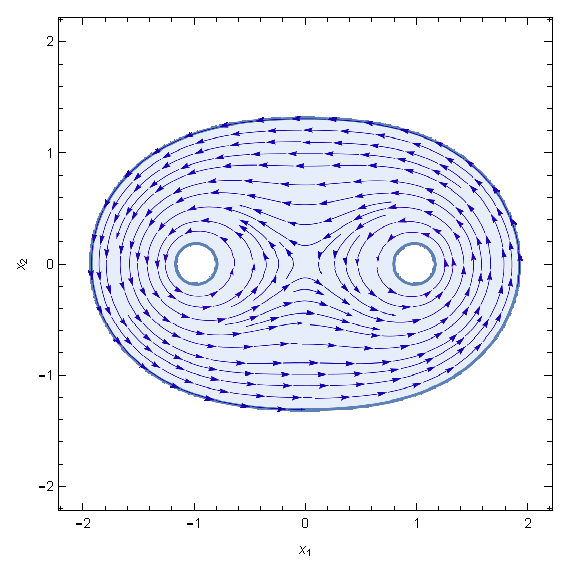
\includegraphics[width=0.7\textwidth]{../Plots/HarmonicVectorFields_gr1.eps}
  \caption{A plot of $u=\nabla^\perp\psi$ in the region $\psi^{-1}\brk*{[-1,1]}$.
    Here $\psi$ is given by equation \eqref{eq:n2:hvf:noInflowNoOutflow}.}
  \label{pl:n2_hvf_noInflowNoOutflow}
\end{figure}

In a second example given by \cite{Wahlen2023} we fix the domain rather than the function.
For this set $\overline{\Omega}=\overline{B_4}\setminus\brk*{B_1(2e_1)\cup B_1(-2e_1)}$ to be the domain.
We then have the system
\begin{equation}
  \begin{aligned}
    \Delta \psi&=0 &&\text{, on }\Omega \\
    \psi&=0 &&\text{, on the outer ring }4S^1 \\
    \psi&=1 &&\text{, on the inner rings }S^1(-2e_1)\cup S^1(2e_1)
  \end{aligned}\label{eq:n2:hvf:roundRegion:noInflowNoOutflow}
\end{equation}
We solve this system numerically and set $u=\nabla^\perp\psi$.
The result is plotted in figure \ref{pl:n2_hvf_roundRegion_noInflowNoOutflow}.
\begin{figure}
  \centering
  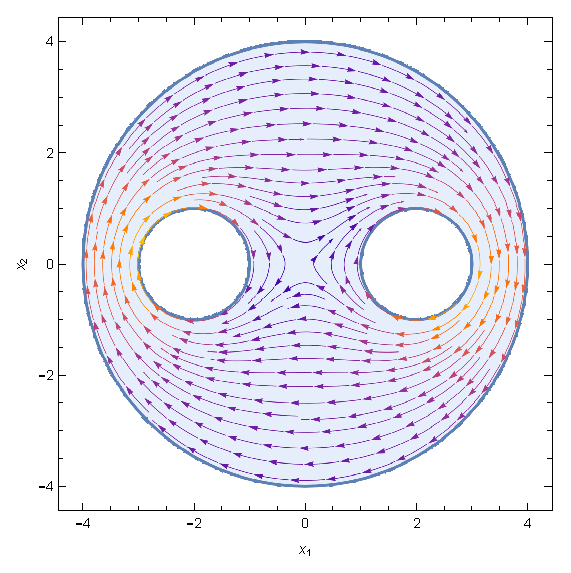
\includegraphics[width=0.7\textwidth]{../Plots/HarmonicVectorFields_gr4.eps}
  \caption{A plot of $u=\nabla^\perp\psi$ where $\psi$ is the numerical solution to
   \eqref{eq:n2:hvf:roundRegion:noInflowNoOutflow}.}
  \label{pl:n2_hvf_roundRegion_noInflowNoOutflow}
\end{figure}

\subsection{An example of inflow on one side and outflow on the other}
In the following we aim to give examples of domains in $d=2$ dimensions for which 
we have inflow on one simply connected boundary component and outflow on another simply connected boundary
component.
For this consider first the stream function
\begin{equation}
  \begin{aligned}
  \psi\colon \R^2\setminus\brk[c]*{-e_1,e_1}&\to\R^2 \\
  x&\mapsto\Phi_2\brk*{x-e_1}+x_1
  \end{aligned}\label{eq:n2:hvf:InflowOutflow:singleHole}
\end{equation}
Figure \ref{pl:n2_hvf_InflowOutflow_asymmetric_single} indicates that $u=\nabla^\perp\psi$ fulfils the
requirements.
\begin{figure}
  \centering
  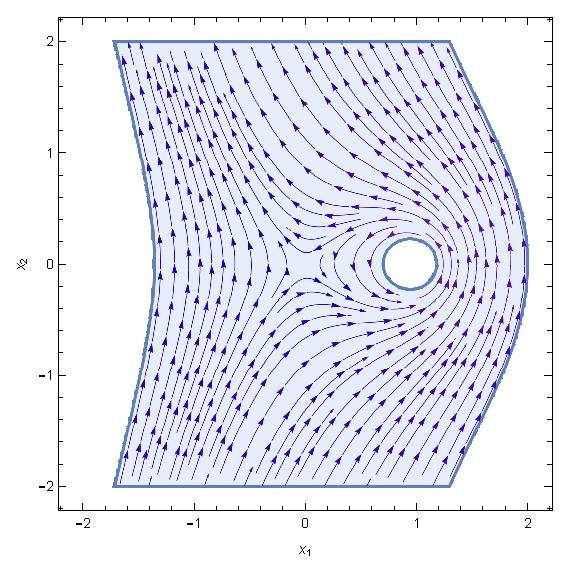
\includegraphics[width=0.7\textwidth]{../Plots/HarmonicVectorFields_gr3.eps}
  \caption{A plot of $u=\nabla^\perp\psi$ in the region $\psi^{-1}\brk*{[-0.5,2]}\cap \R\times[-2,2]$.
  Here $\psi$ is given by equation \eqref{eq:n2:hvf:InflowOutflow:singleHole}.}
  \label{pl:n2_hvf_InflowOutflow_asymmetric_single}
\end{figure}

Now we would like to have a harmonic vector field similar to the example with two holes with
inflow on the one side and outflow on the other. 
For this consider the streamline
\begin{equation}
  \begin{aligned}
  u\colon\R^2\setminus\brk[c]*{-e_1,e_1}&\to\R^2 \\
  x&\mapsto\Phi_2\brk*{x-e_1}-\Phi_2\brk*{x+e_1}+x_1
  \end{aligned}\label{eq:n2:hvf:noInflowNoOutflow:doubleHoles}
\end{equation}
Figure \ref{pl:n2_hvf_InflowOutflow_symmetric_region} indicates that $u=\nabla^\perp\psi$ is the function
we are looking for.
\begin{figure}
  \centering
  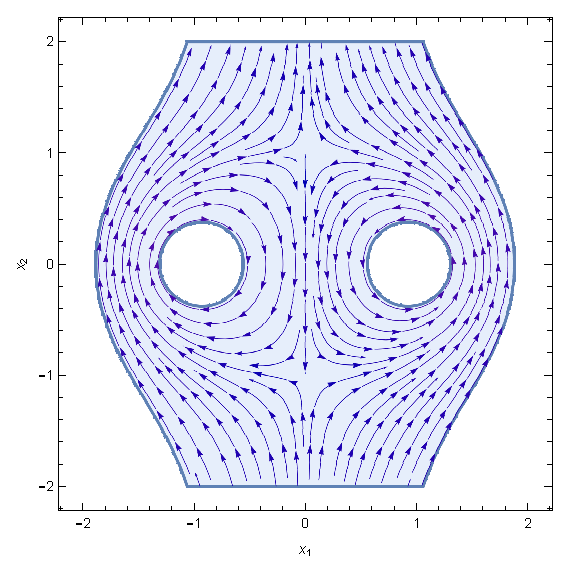
\includegraphics[width=0.7\textwidth]{../Plots/HarmonicVectorFields_gr2.eps}
  \caption{A plot of $u=\nabla^\perp\psi$ in the region $\psi^{-1}\brk*{[-0.7,0.7]}\cap \R\times[-2,2]$.
  Here $\psi$ is given by equation \eqref{eq:n2:hvf:noInflowNoOutflow:doubleHoles}.}
  \label{pl:n2_hvf_InflowOutflow_symmetric_region}
\end{figure}


In another example given by \cite{Wahlen2023} we once again fix the domain rather than the function.
Let $\Omega=B_4\setminus\brk*{B_1(2e_1)\cup B_1(-2e_1)}$ be the domain as before.
We now have the system
\begin{equation}
  \begin{aligned}
    \Delta \psi&=0 &&\text{, on }\Omega \\
    \psi&=0 &&\text{, on the outer ring }4S^1 \\
    \psi&=-1 &&\text{, on the left inner ring }S^1(-2e_1) \\
    \psi&=1 &&\text{, on the right inner ring }S^1(2e_1)
  \end{aligned}\label{eq:n2:hvf:roundRegion:InflowOutflow}
\end{equation}
We solve this system numerically and set $u=\nabla^\perp\psi$.
The result is plotted in figure \ref{pl:n2_hvf_roundRegion_InflowOutflow}.
\begin{figure}
  \centering
  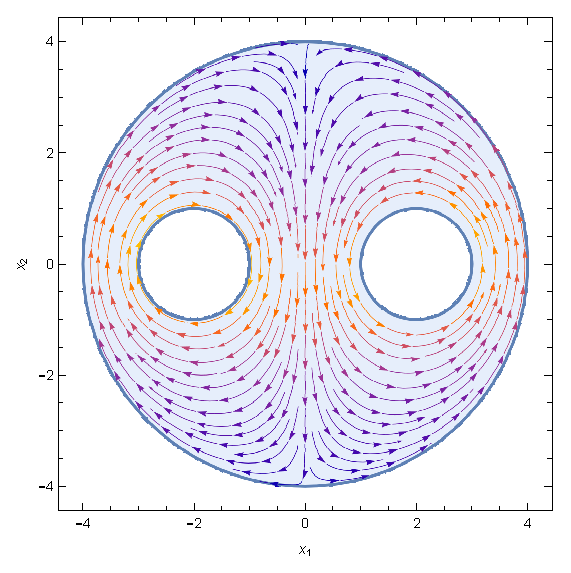
\includegraphics[width=0.7\textwidth]{../Plots/HarmonicVectorFields_gr5.eps}
  \caption{A plot of $u=\nabla^\perp\psi$ where $\psi$ is the numerical solution to
   \eqref{eq:n2:hvf:roundRegion:InflowOutflow}.}
  \label{pl:n2_hvf_roundRegion_InflowOutflow}
\end{figure}
\td{Check the signs of this example. Give explanation for why it works.}

\newpage

\section{Harmonic functions, $d=3$}

\subsection{The cylinder}

The following proof comes from \cite{Wahlen2023}
\begin{proposition}
  Let $\Omega=(0,1)\times B_1\subseteq\R^3$ be the cylinder. Let further $f\colon\overline{\Omega}\to\R$ be regular 
  harmonic with no inflow or outflow on the sides 
  $\partial (0,1)\times B_1$, no outflow on $\brk[c]{0}\times B_1$ and no inflow on $\brk[c]{1}\times B_1$. 
  Then $f$ cannot have a critical point.
\end{proposition}
\begin{proof}
  Assume not. Since
  \begin{align*}
    \Delta(\partial_1f)=\partial_1(\Delta f)=0
  \end{align*}
  we have by the maximum principle that $\partial_1 f$ attains its minimum on the boundary $\Sigma$. Since $\partial_1 f(x)=0$ for some interior point 
  by assumption and $\partial_1 f>0$ on the lids $\brk[c]{x_1=0}\cup\brk[c]{x_1=1}$ there exists a point
  $x\in(0,1)\times S^1$ such that $\partial_1f(x)$ is minimal on $\overline{\Omega}$. But then we have by Hopf's lemma
  that
  \begin{align*}
    0<\nabla (\partial_1f)\cdot n=\partial_1(\nabla f\cdot n)=0\,,
  \end{align*}
  a contradiction.
\end{proof}

\newpage

\subsection{Harmonic vector fields, $d=3$}
We obtain as a quick consequence of the hairy ball theorem
\begin{proposition}
  Let $\Omega$ have Betti numbers $b_0$, $b_1$ and $b_2$.
  Let $u\colon X\to\R$
  be a Morse harmonic vector field without inflow or outflow. Then we have
  \begin{align*}
    b_2\leq b_1\,.
  \end{align*}
\end{proposition}
\begin{proof} 
  Assume not. Since $\Omega$ has $b_2$ bubbles and $b_1$ holes there exists by the pigeon hole
  principle a bubble $\Gamma\subseteq\Sigma$ without a hole. Since $u$ has no inflow or outflow on $\Gamma$ we
  have that the restriction $u\vert_\Gamma\in T\Gamma$ is a vector field on $\Gamma$. Since $u$ is regular
  $u\vert_\Gamma$ does not vanish. But $\Gamma$ is homeomorphic to the Ball in contradiction to the hairy ball theorem.
\end{proof}\ruggedtodo[]{A little more rigour would not harm.}
Mimicking the proof in 2 dimensions we obtain the following proposition.
\begin{proposition}
  Let $X\subset\R^3$ be a compact manifold with corners homeomorphic to the ball $B$.
  Let $f\colon X\to\R$ be a Morse harmonic function. Assume that $\Sigma^-$ is simply connected.
  Then we have that
  \begin{align*}
    M_1=M_2
  \end{align*}
\end{proposition}
\begin{proof}
  As in the two dimensional case we split the domain $\Omega$ with a plane $\Gamma$ such that
  $\partial\Gamma=\gamma=\partial\Sigma^-$.
  Denote the two arising domains $X^+$ and $X^-$ where $\partial X^+=\Sigma^+\cup\Sigma^0\cup\overline{\Gamma}$ and
  $\partial X^-=\Sigma^-\cup\overline{\Gamma}$.
  We can assume that $\Gamma$ is a smooth manifold.
  Since by proposition ?? there are finitely many critical points in $\Omega$
  we can also assume that no interior critical points lie on $\Omega$.
  We now look at a critical point $x$ on $\Gamma$.
  \ruggedtodo[]{Why are there finitely many?}
  We choose the slant at which $\Gamma$ approaches $\gamma$ in such a way that $x$
  is neither an essential critical point of $f$ nor of $-f$.
  \ruggedtodo[]{More details here.}
  We now turn our attention to $X^+$. Since no essential critical points lie on $\Sigma^+$ or
  $\gamma$ it follows for the boundary type numbers that
  \begin{align}
    \mu^+_j=\ind_{j,\Gamma}(f)\,.\label{eq:n2_disproof_morse_muplus}
  \end{align}
  Analogously we have on $X^-$ that
  \begin{align}
    \nu^-_j=\ind_{j,\Gamma}(-f)\,.\label{eq:n2_disproof_morse_numinus}
  \end{align}
  In addition we have that the emergent critical points of $f$ on $X^+$ are the
  entrant critical points of $-f$ on $X^-$, that is
  \begin{equation}
    \begin{aligned}
      \ind_{0,\Gamma}(u)=\ind_{2,\Gamma}(-f) \\
      \ind_{1,\Gamma}(u)=\ind_{1,\Gamma}(-f) \\
      \ind_{2,\Gamma}(u)=\ind_{0,\Gamma}(-f)\label{eq:n2_disproof_morse_relationIndex} 
    \end{aligned}
  \end{equation}
  Using equations \eqref{eq:n2_disproof_morse_muplus}, \eqref{eq:n2_disproof_morse_numinus} and \eqref{eq:n2_disproof_morse_relationIndex}
  we obtain
  \begin{equation}
    \begin{aligned}
      \mu^+_0=\nu^-_2 \\
      \mu^+_1=\nu^-_1 \\
      \mu^+_2=\nu^-_0\label{eq:n2_disproof_morse_relationMuNu}
    \end{aligned}
  \end{equation}
  We observe the Morse inequalities for $f$
  \begin{align}
    M_2^++\mu^+_2-M_1^+-\mu^+_1+\mu^+_0=\chi(X^+)=\chi(X)\,.\label{eq:n2_disproof_morse_morseineqplus}
  \end{align}
  and the Morse inequalities for $-f$
  \begin{align}
    M_1^-+\nu^-_2-M_2^--\nu^-_1+\nu^-_0=\chi(X^-)=\chi(X)\label{eq:n2_disproof_morse_morseineqminus}
  \end{align}
  where the $M_j$ continue to denote the interior type numbers of $f$.
  We now subtract equation \eqref{eq:n2_disproof_morse_morseineqplus} from \eqref{eq:n2_disproof_morse_morseineqminus}
  and insert relations \eqref{eq:n2_disproof_morse_relationMuNu} to obtain
  \begin{align*}
    M_1^--M_2^-+M_1^+-M_2^+=0
  \end{align*}
  from which the claim follows.
\end{proof}
In fact we can give an example for such a function with
simply connected entrant boundary.
\begin{example}[Example of a harmonic vector field with simply connected entrant boundary]
  Consider the domain $X=\overline{B}_r\subseteq\R^3$ with $r>0$ sufficiently large and the harmonic function
  \begin{align*}
    f\colon X&\to\R \\
    x&\mapsto \frac{x_1^2}{2}-\frac{x_1^3}{3}-\frac{x_2^2}{2}+x_1x_2^2+x_2x_3
  \end{align*}
  This induces the harmonic vector field
  \begin{align*}
    u\colon X&\to\R^3 \\
    x&\mapsto\vect{x_1(1-x_1)+x_2^2 \\
      x_2(2x_1-1)+x_3 \\
      x_2}
  \end{align*}
  It follows from setting $u(x)=0$ implies that $x_2=0$
  and then that $x_3=0$ and $x_1\in\brk[c]*{0,1}$. Thus we have that $x\in\brk[c]*{0,e_1}$
  are the sole possible zeroes of $u$. Conversely these are zeroes of $u$.

  Figure \ref{pl:n3_hf_inflowOutflowStagnationPoint_overview}
  indicates that $f$ has the desired properties.
  \begin{figure}
    \centering
    \missingfigure{Some amazing plot showing an overview of f}
    \caption{An plot of the function $u$}
    \label{pl:n3_hf_inflowOutflowStagnationPoint_overview}
  \end{figure}
  \td{complete this section.}
\end{example}

\td{Try to say something about the case without inflow or outflow.}
% And we also obtain
% \tdrewrite{Rewrite this to incorporate the updated notation. And fix the boundary smoothness issues.}
% \begin{proposition}
%   Let $X\subseteq\R^3$ be a compact manifold with corners and Betti numbers $b_0$, $b_1$ and $b_2$.
%   Let $u\colon X\to\R$ be a Morse harmonic vector field without inflow or outflow. Then we have the following relation for
%   the interior type numbers of $u$
%   \begin{align*}
%     M_2=M_1\,.
%   \end{align*}
% \end{proposition}
% \begin{proof}[Sketch of proof.]
%   As in the two dimensional case we cut the domain $\Omega$ with planes $\Gamma$ such that the slit domain is
%   homeomorphic to a ball with bubbles.
%   Since the number of critical points is finite by proposition ??, we can choose $\Gamma$ in such a way
%   that it does not contain any critical points. We also denote the curves at which $\Gamma$ meets $\Sigma$ by 
%   $\gamma_1,\dots,\gamma_{b_1}\subseteq\partial\Gamma$. Note that there are $b_1$ many such curves.

%   Once again by proposition \ref{pr:n2:hvf:simplyConnected} $u$ is the gradient of a harmonic function $u$ on this new domain.
%   $f$ has no critical points on the boundary $\Sigma$ and on the cut boundary it fulfils the conditions
%   \begin{align}
%     \mu_0=\nu_2\qquad \mu_1=\nu_1 \qquad \mu_2=\nu_0 \label{eq:n3:hvf:relationsMuNu}
%   \end{align}
%   by the same reasoning. We now have the Morse inequalities for $f$ and $-f$
%   \begin{align}
%     M_2+\mu_2-b_2-M_1-\mu_1+b_1+\mu_0-b_0=0 \label{eq:n3:hvf:MorseInequalities:1} \\
%     M_1+\nu_2-b_2-M_2-\nu_1+b_1+\nu_0-b_0=0 \label{eq:n3:hvf:MorseInequalities:2}
%   \end{align}
%   It then follows by subtracting equation \eqref{eq:n3:hvf:MorseInequalities:2} from \eqref{eq:n3:hvf:MorseInequalities:1}
%   and using relations \eqref{eq:n3:hvf:relationsMuNu} that
%   \begin{align*}
%     2\brk*{M_2-M_1}=0\,.
%   \end{align*}
% \end{proof}\ruggedtodo[]{Introduce Morse inequalities for $-f$.}


\newpage

\subsection{Harmonic functions, $d=4$} 
Define the harmonic function 
\begin{align*}
  f\colon B_1\subseteq\R^4&\to \R \\
  x &\mapsto x_1^2+x_2^2-x_3^2-x_4^2\,.
\end{align*}
This has a stagnation point at the origin. We now claim that the sets $\Sigma^+$ and $\Sigma^-$ are both simply connected, i.e.\
we have a tube in $\R^4$ with throughflow and a stagnation point.

\begin{proof}
To prove this claim we observe that the boundary $\partial B_1$ can be parametrised by the coordinates $\bx = (x_2,x_3,x_4)$
for which we have $\abs{\bx}\leq 1$. By the condition
\begin{align}
  \sum_i x_i^2 = 1\label{eq:n4:ball}
\end{align}
on the boundary $\partial B_1$ we have that $x_1$ is then uniquely determined up to sign. Thus we have have defined parametrisations
\begin{align}
  \begin{aligned}\phi_\pm\colon B_1\subseteq\R^3&\to\R \\
  \bx&\mapsto x\text{ such that } \pm x_1\geq0
  \end{aligned}\label{eq:n4:parametrisation}
\end{align}
with inverses $\psi_\pm = \brk*{\phi_\pm}^{-1}$.
We now calculate the gradient of $f$
\begin{align*}
  \nabla f = 2\vect{x_1 & x_2 & -x_3 & -x_4}^\top
\end{align*}
and the normal to $\partial B_1$
\begin{align*}
  n = \vect{x_1 & \cdots & x_4}^\top\,.
\end{align*}
Thus we have $x\in\Sigma^\pm$ iff
\begin{align*}
  0<\pm \nabla f\cdot n = \pm 2\brk*{x_1^2+x_2^2-x_3^2-x_4^2}
\end{align*}
Using condition \eqref{eq:n4:ball} we obtain the equivalent condition
\begin{align*}
  0<\pm 1-2\brk*{x_3^2+x_4^2}
\end{align*}
Define the cylinder
\begin{align*}
  C = \brk[c]*{\bx\in \R^3\colon x_3^2+x_4^2<1/2} = \R\times B_{1/\sqrt{2}}
\end{align*}
If we return to our parametrisation \eqref{eq:n4:parametrisation} we see that we have $\bx\in B_1\cap C$ iff
$\phi_\pm(x)\in \Sigma^+$ and hence 
\begin{align*}
  B_1\cap C=\psi_\pm\brk*{\Sigma^+}\,.
\end{align*}
Analogously  we have 
\begin{align*}
  B_1\setminus C=\psi_\pm\brk*{\Sigma^-}\,.
\end{align*}
The claim then follows from the fact that $\phi$ is a homeomorphism onto its image and $x_1=0$ is 
equivalent to $\bx\in \partial B_1\subseteq \R^2$. The situation is depicted in figure \ref{fi:n4_sigma}.

\td{Check that the transition at the boundary is legal.}
\begin{figure}[h]
  \centering
  \def\svgwidth{0.7\textwidth}
  \input{../Figures/n4_sigma.pdf_tex}
  \caption{Visualisation of the situation.}
  \label{fi:n4_sigma}
\end{figure}
\end{proof}


% \printnomenclature

\glsaddall
\printunsrtglossary[type=symbols,style=long]


% TODO: potentially add Irwin, smooth dynamical systems
% \section{Bibliography}
\nocite{*}
\td{Change Gamelin to Lang, complex analysis}
%Main source
%\printbibliography[heading=none, keyword={main}]
%\noindent Other sources
\printbibliography


\end{document}